%
%  Simulations
% =============
%

\chapter{Simulation Analysis}
\label{Ch:SimA}

This chapter outlines some of the key considerations and calculations performed on the data sets generated in these simulations.
Analysis tools were developed in MATLAB for both OSIRIS and QuickPIC data sets.
These are available online, and are described in more detail in Appendix~\ref{Apx:DA}.

% ================================================================================================================================ %
\section{Extracting Twiss Parameters from Particle Arrays}
\label{SimA:EnTwiss}

Both OSIRIS and QuickPIC dump the macro particles as large arrays of six-dimensional data, providing each particle's position and momentum vector.
QuickPIC uses equally weighted macro particles, greatly simplifying the analysis.
OSIRIS, however, uses weighted macro particles, so the weights need to be considered when performing the statistical calculations.
Additional statistical functions were added to MATLAB's own to perform these weighted calculations (see Appendix~\ref{Apx:DA}).

To study the collective motion of particles it is useful to calculate the bunch total emittance in terms of the RMS value or standard deviation of its particles.
Equation~\ref{EQ:EmittFull} from Section~\ref{Int:BPI:EnTwiss} can be rewritten in terms of the statistical distributions of its particles such that
\begin{equation}
    \epsilon = \sqrt{\gamma\sigma_{x}^{2} + 2\alpha\sigma_{x}\sigma_{x^{\prime}} + \beta\sigma_{x^{\prime}}^{2}}, \label{EQ:Emitt}
\end{equation}
where the angle of the $i$-th particles can be taken from its momentum
\begin{equation}
    x_{i}^{\prime} = \frac{p_{i,x}}{p_{i,z}}.
\end{equation}

For a set of macro particles, the geometric emittance can be calculated directly by taking the covariance matrix of the $x$ and $x^{\prime}$ vectors
\begin{equation}
    \mathbf{T} = \mathrm{cov}\left(\mathbf{x}, \mathbf{x}^{\prime}\right), \label{EQ:ECalc1}
\end{equation}
and then taking the square root of its determinant
\begin{equation}
    \epsilon = \sqrt{\mathrm{det}\left(\mathbf{T}\right)}. \label{EQ:ECalc2}
\end{equation}
The Twiss parameters can be extracted from the matrix $\mathbf{T}$ as well:
\begin{equation}
    \alpha = \mathrm{T}_{12}/\epsilon, \quad
    \beta  = \mathrm{T}_{11}/\epsilon, \quad
    \gamma = \mathrm{T}_{22}/\epsilon.
\end{equation}

% ================================================================================================================================ %
\section{A Measure for Beam Quality}
\label{SimA:QTilde}

For the emittance study in Publication~\ref{Pub:BL17} it was necessary to define a convenient unit for the quality of the accelerated bunch in terms of emittance evolution in regions along the bunch length.
In the quasi-linear plus non-linear regime this publication investigates, emittance growth only occurs at the head of the bunch.
However, the region of emittance growth varies when parameters such as charge and bunch size changes.
In the study we defined a parameter that quantifies emittance preservation,
\begin{equation}
    \tilde{Q} = \frac{1}{N} \sum_{m=0}^{M} \sum_{n=0}^{N} Q_{m+n}\,\chi(\xi_{m},N),\label{EQ:BeamQ}
\end{equation}
where $M$ is the number of longitudinal grid slices of length $\Delta\xi$ which contains macro particles for the witness bunch, and with corresponding coordinate $\xi_{m}$.
$N$ is the number of such slices to average over.
And $\chi(\xi_{m},N)$ is the step function
\begin{equation}
    \chi(\xi_{i},N) =
    \begin{cases}
        1, & \frac{\epsilon_{i} - \epsilon_{0}}{\epsilon_{0}} \leq 5\% \\
        0, & \frac{\epsilon_{i} - \epsilon_{0}}{\epsilon_{0}} > 5\%
    \end{cases}
    \quad\mathrm{for~}\epsilon_{i}\mathrm{~over~the~interval}\quad
    [\xi_{i}, \xi_{i} + N\Delta\xi],
\end{equation}
where $\epsilon_{i}$ is the emittance as defined by Equations~\ref{EQ:ECalc1} and~\ref{EQ:ECalc2} for a set of macro particles within the interval $\xi_{i}$ to $\xi_{i} + N\Delta\xi$, and $\epsilon_{0}$ is the initial emittance defined in the simulation input file.
For the studies included in Publication~\ref{Pub:BL17},
\begin{equation}
    M = \left\lfloor \frac{10\sigma_{z}}{\Delta\xi} \right\rceil, \quad
    N = 4.
\end{equation}
The first slice coordinate for the iterator $m$ is
\begin{equation}
    \xi_{m=0} = \mu_{\mathrm{eb}} - 5\sigma_{z,\mathrm{eb}} - 0.5\Delta\xi,
\end{equation}
where $\mu_{\mathrm{eb}}$ is the longitudinal centre of the bunch.

The quantity $\tilde{Q}$ is thus the total charge that retains its initial emittance within a limit of $5\%$ growth.
The emittance is calculated with a moving window of $4$ grid cells over $\pm 5\sigma_z$ of the bunch.

\paragraph{Note:} This method may yield a misleading result if the Twiss parameter $\alpha$ varies too much along the length of the bunch.
That is, a rotation of the phase-space ellipse, see Figure~\ref{Fig:BPI:Twiss}.
The emittance can be locally small and qualify for the $5\%$ criterion, even if the total emittance of the region included in $\tilde{Q}$ is not.
This can easily be checked after the seemingly optimal region of the bunch is known by verifying that its total emittance does not exceed the same criterion.

% ================================================================================================================================ %
%  Full Scale Studies
% ================================================================================================================================ %
\section{Full Scale Studies}
\label{SimA:FullScale}

A total of 38 simulations of a full AWAKE proton bunch, with and without an injected electron bunch, were run.
As can be seen from Table~\ref{T:SimCost}, these simulations took an average of over $11\,000$ CPU hours each.
The simulation parameters used for these studies are described in Section~\ref{Sim:PBeam}.

The purpose of the full scale studies were mainly to develop some familiarity with OSIRIS, but also to study the properties of the self-modulated beam in order to make a reasonable approximation of it for the later pre-modulated studies (see Section~\ref{Sim:PBPreMod}).

The modulation period of the self-modulated beam was checked with Fast Fourier Transform (FFT)~\cite{van_loan:1992}.
The FFT revealed that the core modulation frequency is indeed the characteristic frequency of the plasma as presented in Publication~\ref{Pub:IPAC15}.

\begin{figure}[hbt]
    \centering
    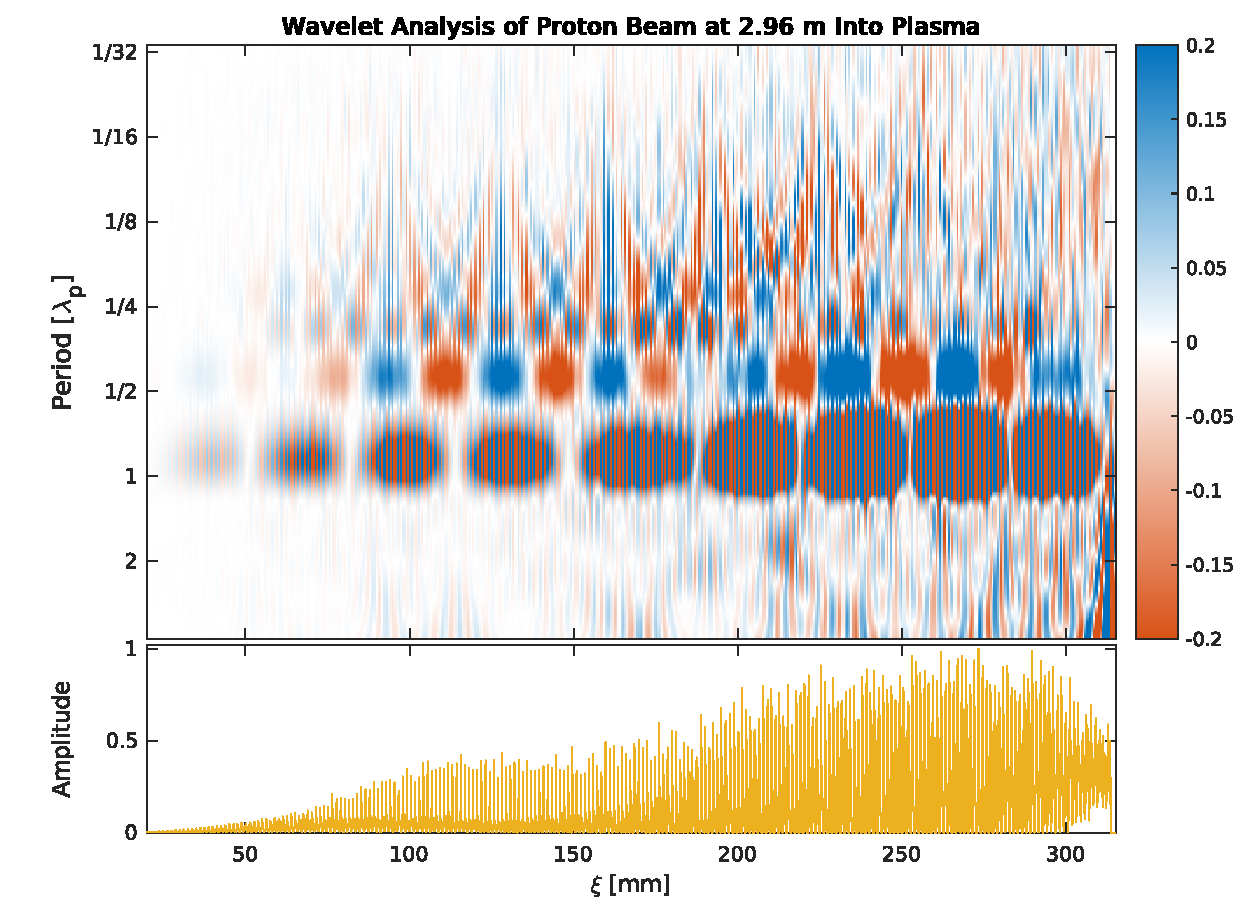
\includegraphics[width=1.0\linewidth]{figures/PBSMIWavelet}
    \caption{\label{Fig:SimA:Wavelet}
        A wavelet analysis of the beam shown in Figure~\ref{Fig:Sim:SMI}, at the same position in the plasma, using Morlet wavelet analysis~\cite{torrence:1998}.
        The horizontal axis shows the position~$\xi$ in the simulation box.
        The vertical axis shows the Fourier period in units of the plasma wavelength~$\lambda_p$.
        This density plot is the absolute value of the complex wavelet data, showing clearly the peak in frequency in the area around the plasma wavelength.
        The colour axis is saturated at amplitude $1$ in order to show the fine structure of the harmonics.
        The contour plot overlay shows the full range of the density data in steps of $0.5$.
    }
\end{figure}

A wavelet analysis was also performed using a Morlet wavelet analysis~\cite{goupillaud:1984,bernardino:2005}.
The wavelet adds some additional information about the modulation frequency as a function of position along the modulated beam of micro bunches.
Such a plot is shown in Figure~\ref{Fig:SimA:Wavelet} where the proton bunch has propagated through about $3\unit{m}$ of plasma.
The figure shows the magnitude of the wavelet analysis data~\cite{lee:1994}, and the amplitude indicates that the density variation is the highest at the front of the bunch (compare with initial profile in Figure~\ref{Fig:Sim:SMI}).

The frequency of the pre-modulated beam was slightly adjusted such that the FFT profiles matched that of the full scale SMI simulations~\cite{berglyd_olsen:2015}.

Both FFT and Wavelet analysis tools were implemented in the \textit{OsirisAnalysis} package described in Section~\ref{Tools:OAAdd}.

% ================================================================================================================================ %
%  Beam Loading and Energy Spread
% ================================================================================================================================ %
\section{Beam Loading and Energy Spread}
\label{SimA:BLoad}

When the parameters of the self-modulated bunch had been established, and the pre-modulated studies set up as laid out in Section~\ref{Sim:PBPreMod}, the evolution of the electron bunch became the main focus.
Of particular interest in the early studies was the beam loading of the electron witness bunch on the longitudinal wakefields, as well as its energy spread as it propagated through the plasma section.

The transverse size of the bunch was initially chosen to be $\sigma_{x,y}=105\unit{\mu m}$, see Table~\ref{T:AWAKERuns}.
This is the size initially proposed for Run~1.
The longitudinal size was chosen to be $\sigma_{z}=40\unit{\mu m}$ for the studies included in Publication~\ref{Pub:IPAC15}, but several lengths were tested in simulations.

\begin{figure}[hbt]
    \centering
    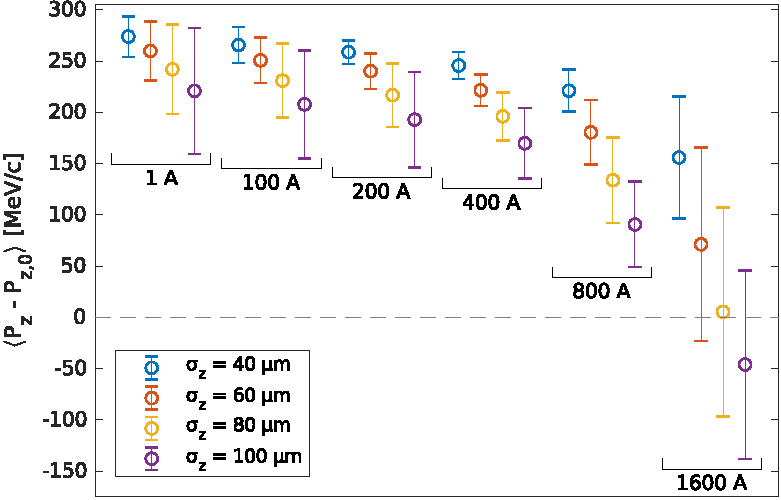
\includegraphics[width=0.625\linewidth]{figures/NAPACEGainSpreadScan}
    \caption{\label{Fig:SimA:BLoadScan}
        A parameter scan for the 26 bunch pre-modulated studies where six different bunch currents and four different bunch lengths were considered.
        The energy gain $P_{z} - P_{z,0}$ after $1.1\unit{m}$ of plasma is shown with the error bars representing the RMS energy spread.
        The figure is presented in Publication~\ref{Pub:NAPAC16} and in Adli \etal~\cite{adli:2016a}.
    }
\end{figure}

Tuning the longitudinal size is essential.
On the one hand, a short bunch positioned at an optimal accelerating phase ensures a low energy spread as all electrons see close to the same accelerating field.
On the other hand, a long bunch is capable of holding a larger charge without the charge density becoming critical.
The bunch length and charge the field is able to support can be improved by tuning the parameters such that the field is flat in the region where the witness bunch is located, as discussed in Section~\ref{Int:BPI:BLoad}.

The initial studies showed that $\sigma_{z} = 40-60\unit{\mu m}$ is a good compromise between having a short enough bunch to stay within the accelerating region of the accelerating wakefield, $\approx \lambda_{pe}/4$ (see Section~\ref{Int:BPI:BLoad}), and a long enough bunch to contain a reasonable amount of electrons without overloading the wakefield.
A larger parameter scan was performed for Publication~\ref{Pub:NAPAC16}, and was presented as a contributing talk at North American Particle Accelerator Conference in Chicago in 2016.
It was also included in~\cite{adli:2016a}.
The main results of this parameter scan is shown in Figure~\ref{Fig:SimA:BLoadScan}.

% ================================================================================================================================ %
%  Emittance Evolution
% ================================================================================================================================ %
\section{Emittance Evolution}
\label{SimA:Emitt}

Achieving a large energy gradient and a low energy spread while maximising charge is a compromise between parameters~\cite{berglyd_olsen:2018}.
High charge density affects beam loading which, when mismatched, may lead to increased energy spread.
An overloaded accelerating field will also reduce energy gain through the accelerating region.
In addition to these considerations, we also seek to preserve the initial emittance and avoid emittance growth.

\begin{figure}[hbt]
    \centering
    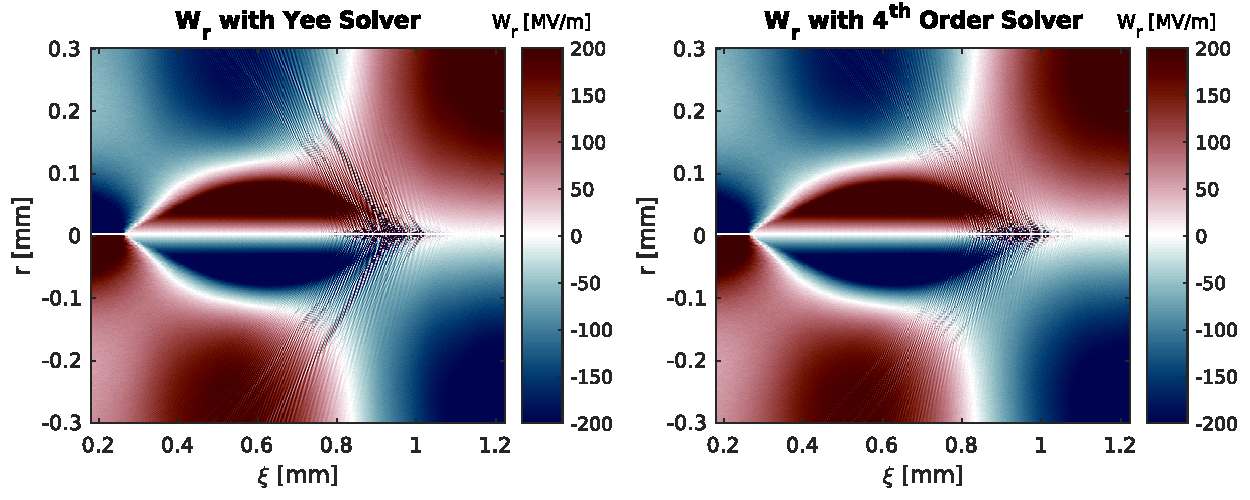
\includegraphics[width=0.999\linewidth]{figures/EMFSolverNoise}
    \caption{\label{Fig:SimA:EMFNoise}
        The radial wakefields $W_r$ for two test simulations of a high density electron bunch.
        The numerical noise generated by the electromagnetic field solvers is clearly seen as additional short period ``wake ripples''.
        The data is taken at the entry into the plasma region, and shows results for both the Yee solver and the slightly better 4\ts{th} order solver in OSIRIS 3.0.
        Both simulations were run without smoothing.
        Tests with smoothing of the fields had some effect.
        The colour axis is truncated to show the structure of the noise.
        The peak of the noise is $3-4$ times higher.
    }
\end{figure}

The simulations for Publication~\ref{Pub:NAPAC16} did not focus on emittance, and were therefore run with OSIRIS~3.0, which is a full PIC code (see Appendix~\ref{Apx:PIC}).
However, due to the numerical noise in the electromagnetic field solver associated with full PIC codes, as also discussed in the appendix, we opted to use QuickPIC at this stage.
Before we moved to QuickPIC, we ran a number of test simulations probing the scale of the noise issue.
OSIRIS provides a number of solvers and filters to minimise the issue, but as illustrated in Figure~\ref{Fig:SimA:EMFNoise}, it was too large of an issue for our specific case with a high density electron bunch.

% ================================================================================================================================ %
\subsection{The Quasi-Linear Regime}
\label{SimA:QLin}

As AWAKE operates in the quasi-linear regime, all the simulations were run with a plasma density matching the expected conditions in the experiment's vapour cell for Run~2.
The quasi-linear regime has the benefit of combining near radially uniform accelerating fields with a nearly non-linear wake (see Section~\ref{Int:BPI:QLin}).

\begin{figure}[hbt]
    \centering
    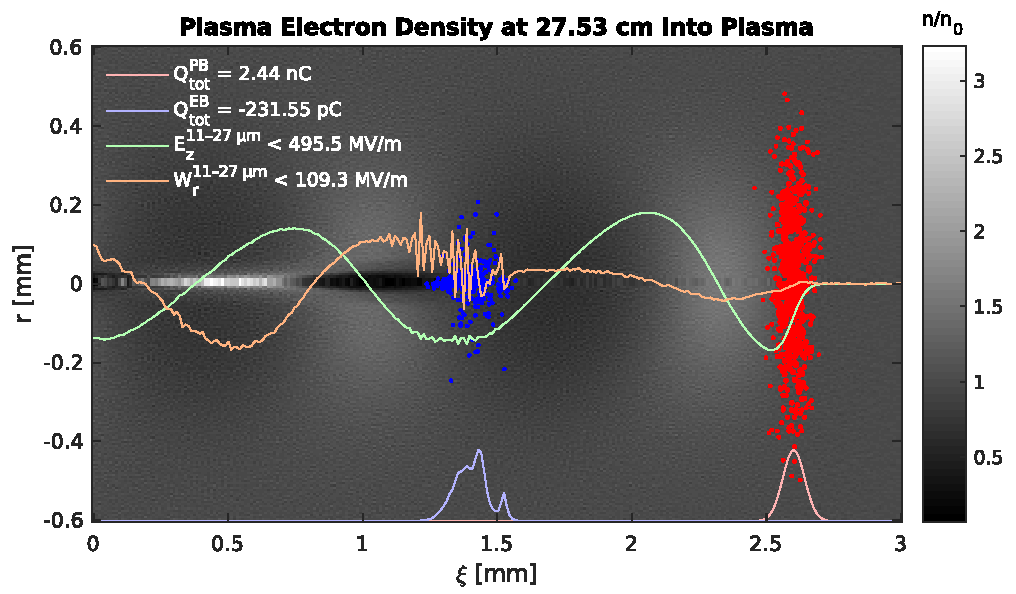
\includegraphics[width=0.8125\linewidth]{figures/NAPACPlasmaDensity}
    \caption{\label{Fig:SimA:NAPACPD}
        Loading of the field after for a $500\unit{A}/60\unit{\mu m}$ electron bunch.
        A sample of electrons can be seen in blue, and protons in red, as well as their respective projections at the bottom.
        The $E_z$ and $W_r$ wakefields are also shown in green and brown respectively.
        The figure is recreated from Publication~\ref{Pub:NAPAC16}.
    }
\end{figure}

However, in the presence of a high density electron witness bunch, a secondary bubble forms behind it.
This bubble is typically non-linear.
The simulations for Publication~\ref{Pub:NAPAC16} showed that this was the case for our optimal range of bunch size and density.
One such example is shown in Figure~\ref{Fig:SimA:NAPACPD}, taken from Publication~\ref{Pub:NAPAC16}.
We labelled this setup as the \textit{Quasi-Linear + Non-Linear Case}.

% ================================================================================================================================ %
\subsection{The Quasi-Linear + Non-Linear Case}
\label{SimA:QLinNonLin}

An electron witness bunch matched to the typical AWAKE plasma density will be, as discussed in Section~\ref{Int:BPI:Match}, very narrow.
At a typical normalised emittance of $2.0\unit{\mu m}$, the matched bunch $\sigma_r$ is $5.25\unit{\mu m}$.
Even at low charge and at the upper limit in terms of bunch length, the wakefields of such a bunch will quickly reach the non-linear regime.
In the base case used in the beam loading study in Publication~\ref{Pub:BL17}, the peak density of the bunch $n_b/n_0 > 35$, is well beyond the saturation level of the bubble that occurs when $n_b/n_0 > 10$ \cite{lu:2005}.

\begin{figure}[hbt]
    \centering
    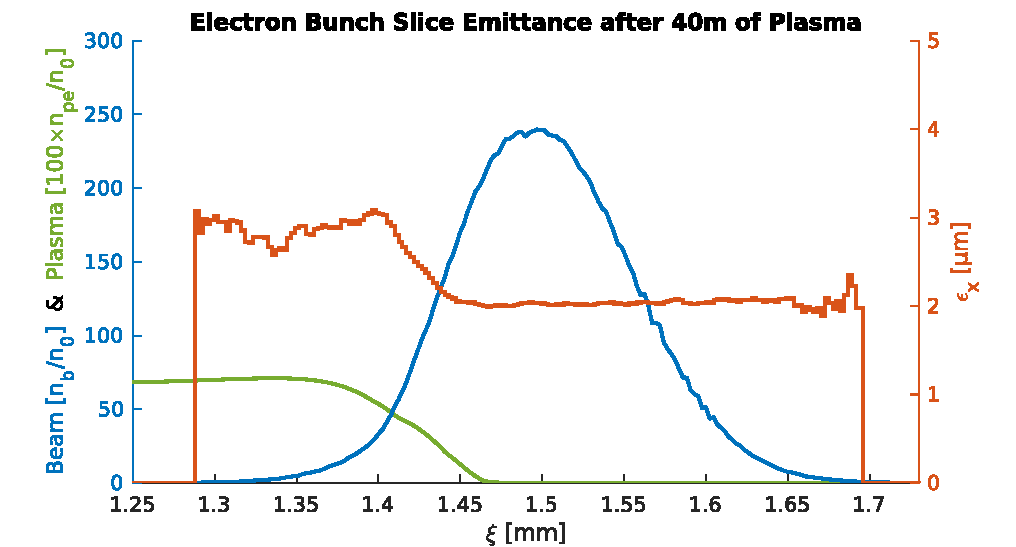
\includegraphics[width=0.8125\linewidth]{figures/40mSliceEmittance}
    \caption{\label{Fig:SimA:BL17Emitt}
        Emittance of an electron bunch along the $\xi$ axis.
        The emittance of the slices are computed with a moving average window of four grid cells or $\approx 9.4\unit{\mu m}$, and shown in red.
        The corresponding electron witness bunch density is shown in blue and the plasma electron density in green.
        The bunch is shown after having propagated through $40\unit{m}$ of plasma.
        The initial emittance for this simulation was $2\unit{\mu m}$, and there is no significant emittance growth in the region in the bunch's own bubble.
        The bunch travels towards the left of the figure.
    }
\end{figure}

The implication here is that there is an additional beneficial effect of loading the accelerating field with as much charge as it will allow without overloading it.
The resulting non-linear wake driven by the head of the bunch, which will see emittance growth due to the quasi-linear conditions of the proton wake, ensures that the rest of the bunch sees a strong focusing force from the pure ion column preventing further emittance growth.
As the electron bunch gains energy, its transverse size will decrease as its emittance is preserved as $\sigma_{r} = \sqrt{\emitN\beta}$~\cite{wille:2001}.
This is clearly shown in Figure~\ref{Fig:SimA:BL17Emitt}, generated from the same data as presented in Publication~\ref{Pub:BL17}.
The head of the bunch sees an emittance growth to about $3\unit{\mu m}$, while the bulk of the bunch sees none.

With this setup there is a range of parameters that needs fine tuning.
In Publication~\ref{Pub:BL17}, we performed a number of parameter scans, attempting to maximise beam quality as defined in Equation~\ref{EQ:BeamQ}.

% ================================================================================================================================ %
\subsection{Convergence Scan}
\label{SimA:Converge}

For the large parameter scans performed for Publication~\ref{Pub:BL17}, it was necessary to verify that the results were not dependant on grid resolution.
The radial wakefields within the plasma bubble are linear, but so are the fields within one grid cell as they are interpolated on the grid.
The effect of linear focusing could thus be an artefact of resolution.
That is especially true in the case where the grid cells were only a factor $2.5$ smaller than the bunch $\sigma_{x,y}$, and thus the bubble radius also small.

\begin{table}[hbt]
    \centering
    \caption{Convergence results for a reference simulations for Publication~\ref{Pub:BL17}.
    The reference bunch has a charge of $250\unit{pC}$, and the emittance tolerance criterion for the $\tilde{Q}$ parameter is $5\%$ (see Section~\ref{SimA:QTilde}).}
    \label{T:Converg}
    \begin{tabularx}{132mm}{Xl d{1}l d{1}l d{1}l}
        \rowcolor{tblhead}
        \texthh{Length} & \texthh{Param.}
            & \multicolumn{2}{c}{\texthh{1024$\times$1024}}
            & \multicolumn{2}{c}{\texthh{2048$\times$2048}}
            & \multicolumn{2}{c}{\texthh{4096$\times$4096}} \\
        \hline
                         & $\tilde{Q}$ &  213.9 & $\unit{pC}$  &  206.9 & $\unit{pC}$  &  213.1 & $\unit{pC}$  \\
        $40\unit{\mu m}$ & MEAN$(E)$   & 2263   & $\unit{MeV}$ & 2233   & $\unit{MeV}$ & 2247   & $\unit{MeV}$ \\
                         & STD$(E)$    &  267.4 & $\unit{MeV}$ &  250.4 & $\unit{MeV}$ &  261.5 & $\unit{MeV}$ \\
        \hline
                         & $\tilde{Q}$ &  221.6 & $\unit{pC}$  &  222.0 & $\unit{pC}$  &  222.1 & $\unit{pC}$  \\
        $60\unit{\mu m}$ & MEAN$(E)$   & 2346   & $\unit{MeV}$ & 2336   & $\unit{MeV}$ & 2333   & $\unit{MeV}$ \\
                         & STD$(E)$    &  166.8 & $\unit{MeV}$ &  165.0 & $\unit{MeV}$ &  165.5 & $\unit{MeV}$ \\
        \hline
                         & $\tilde{Q}$ &  229.9 & $\unit{pC}$  &  226.9 & $\unit{pC}$  &  224.8 & $\unit{pC}$  \\
        $80\unit{\mu m}$ & MEAN$(E)$   & 2378   & $\unit{MeV}$ & 2379   & $\unit{MeV}$ & 2368   & $\unit{MeV}$ \\
                         & STD$(E)$    &  120.0 & $\unit{MeV}$ &  117.6 & $\unit{MeV}$ &  119.1 & $\unit{MeV}$ \\
    \end{tabularx}
\end{table}

% ================================================================================================================================ %
\section{Summary of Simulation Studies}
\label{SimA:Summary}

Table~\ref{T:SimCost} gives an overview of the simulation studies done as a part of the thesis work.
Nearly all of the 1.5 million CPU hours used for these simulations were done using the super computer \textit{Abel}, located at the the USIT department at the University of Oslo and owned by the University of Oslo and The Norwegian Metacenter for Computational Science.
Project code for the computing access was \texttt{nn9303k}.

Some of the simulations were also run on the computing cluster \textit{Smaug} hosted at the Department of Physics and maintained by the students at Computational Physics.

\begin{table}[hbt]
    \centering
    \caption{Overview of total simulation cost. $97\%$ of the simulations were run on the supercomputer \textit{Abel}, on Oct Core Intel Xeon E5-2670 CPUs. The remainder were run on older nodes with Quad Core AMD Opteron 2354 CPUs.}
    \label{T:SimCost}
    \begin{tabularx}{\textwidth}{Xlrrr}
        \rowcolor{tblhead}
        \texthh{Topic of Studies}                & \texthh{Code} & \texthh{Count} &     \texthh{CPU Time} &  \texthh{Average} \\
        \hline
        Preliminary studies (mostly testing)     & OSIRIS        &           $21$ &    $266\,599\unit{h}$ & $12\,695\unit{h}$ \\
        Full length AWAKE proton bunch studies   & OSIRIS        &           $38$ &    $440\,583\unit{h}$ & $11\,594\unit{h}$ \\
        Pre-modulated beam studies$^{1}$         & OSIRIS        &          $144$ &    $319\,093\unit{h}$ &  $2\,216\unit{h}$ \\
        3D reference studies                     & OSIRIS        &           $23$ &    $245\,974\unit{h}$ & $10\,695\unit{h}$ \\
        Single drive bunch studies$^{2}$         & OSIRIS        &          $124$ &     $47\,837\unit{h}$ &     $386\unit{h}$ \\
        Beam loading and emittance studies$^{3}$ & QuickPIC      &          $293$ &    $369\,887\unit{h}$ &  $1\,262\unit{h}$ \\
        \hline
        \rowcolor{tblfoot}
        Total                                    &               &          $657$ & $1\,479\,350\unit{h}$ &  $2\,252\unit{h}$ \\
        \multicolumn{5}{p{50mm}}{\footnotesize
            $^{1}$ Main studies for Publication \ref{Pub:IPAC15} \newline
            $^{2}$ Main studies for Publication \ref{Pub:NAPAC16} \newline
            $^{3}$ Main studies for Publication \ref{Pub:BL17} \newline
        }
    \end{tabularx}
\end{table}

% ================================================================================================================================ %
